\documentclass[aspectratio=169]{beamer}

% Serbian Latin characters support
% Compiled with Tectonic (XeTeX engine): use fontspec for full Unicode (š, č, ć, ž, đ).
% Do NOT load inputenc/fontenc/lmodern - those are pdfTeX-era and drop diacritics.
\usepackage{fontspec}

% Graphics and tables
\usepackage{graphicx}
\usepackage{booktabs}
\usepackage{amsmath}

% Theme - clean and professional
\usetheme{Madrid}
\usecolortheme{default}

% Serbian language settings
\renewcommand{\figurename}{Slika}
\renewcommand{\tablename}{Tabela}

% Custom footline with slide numbers
\setbeamertemplate{footline}[frame number]
\setbeamertemplate{navigation symbols}{}

\title[Poređenje MCNN i CSRNet modela]{Poređenje MCNN i CSRNet modela\\za brojanje ljudi u gužvi}
\author[Dimitrijević, Kutlešić]{Uroš Dimitrijević \and Miloš Kutlešić}
\institute[FTN]{Projektni rad iz predmeta Mašinsko učenje}
\date{}

\begin{document}

% Slide 1: Title
\begin{frame}
    \titlepage
\end{frame}

% Slide 2: Introduction
\begin{frame}{Uvod i motivacija}
    \begin{itemize}
        \item \textbf{Problem}: Automatsko brojanje ljudi na slikama gustih gužvi
        \item \textbf{Zašto ne detekcija objekata?}
        \begin{itemize}
            \item Jaka okluzija (prekrivanje) u gustim scenama
            \item Mali objekti, teško razlikovanje pojedinaca
            \item Previše instanci za bounding box pristup (npr. YOLO)
            \item Segnmentacija instanci takođe nepovoljna: ljudi se u gužvi \emph{spajaju} u jednu regiju, maska po osobi je preskupa za anotiranje --- dataset daje samo tačke (glave)
        \end{itemize}
        \item \textbf{Rešenje}: Regresija mape gustine (density map)
        \begin{itemize}
            \item Model uči "koliko je gusta svaka oblast", ne "gde je svaka osoba"
            \item Ukupan broj = integral (suma) mape gustine
        \end{itemize}
    \end{itemize}
\end{frame}

% Slide 3: Theory - Density Maps
\begin{frame}{Teorijska osnova: Mape gustine}
    \begin{columns}[T]
        \column{0.55\textwidth}
        \begin{itemize}
            \item Svaka anotacija (glava) se modeluje Gausovim kernelom:
            \[
                \begin{aligned}
                    F(x) &= \sum_{i=1}^{N} \delta(x-x_i) * G_{\sigma_i}(x) \\
                    G_{\sigma}(x) &= \frac{1}{2\pi\sigma^{2}}\, e^{-\|x\|^{2}/(2\sigma^{2})}
                \end{aligned}
            \]
            \item \textbf{Broj osoba} = $\sum$ vrednosti piksela mape gustine
            \item Fiksna $\sigma=15$ (kontrolisano poređenje) vs. adaptivna (u daljem radu)
            \item Prednost: uči distribuciju gužve, robustno na okluzije
        \end{itemize}
        
        \column{0.42\textwidth}
        \begin{center}
            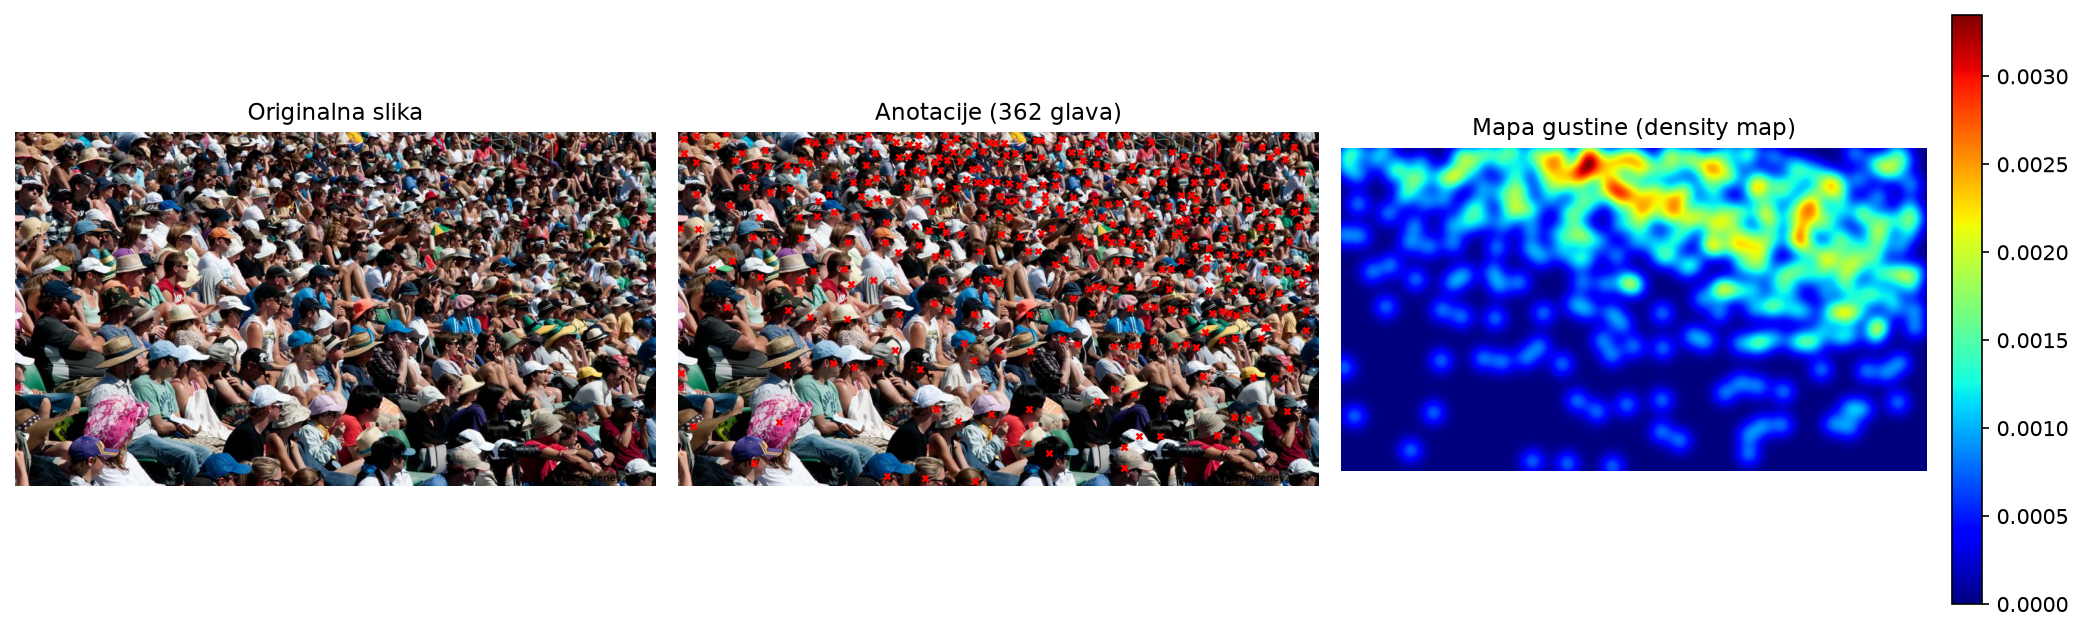
\includegraphics[width=\textwidth]{figures/density_map_illustration.png}\\[0.2em]
            {\scriptsize Slika $\rightarrow$ anotacije $\rightarrow$ mapa gustine}\\[0.4em]
            {\small Diskretni Gausov kernel:}\\[0.2em]
            $\dfrac{1}{273}\begin{bmatrix}
                1 & 4 & 7 & 4 & 1\\
                4 & 16 & 26 & 16 & 4\\
                7 & 26 & 41 & 26 & 7\\
                4 & 16 & 26 & 16 & 4\\
                1 & 4 & 7 & 4 & 1
            \end{bmatrix}$\\[0.4em]
            {\scriptsize težine oko tačke glave, $\sigma \approx 1.05$; zbir težina $= \frac{273}{273} = 1$ --- svaka glava doda tačno 1 osobu}
        \end{center}
    \end{columns}
\end{frame}

% Slide 4a: Architecture - MCNN
\begin{frame}{Arhitektura: MCNN (Zhang et al., 2016)}
    \begin{columns}[T]
        \column{0.54\textwidth}
        \begin{itemize}
            \item \textbf{Problem skale}: bliske glave $\sim$30$\times$30 px, daleke $\sim$5$\times$5 px --- jedan filter ne pokriva obe
            \item \textbf{Rešenje}: tri paralelne grane, svaka specijalizovana za jednu skalu
            \item \textbf{Fuzija}: konkatenacija kanala + 1$\times$1 konv. uči gde da veruje kojoj grani (gusta gužva $\rightarrow$ sitni filteri)
            \item Učenje od nule (from scratch), bez pretreniranog backbone-a
            \item \textbf{Slabosti}: gubitak rezolucije kroz pooling ($\frac{H}{4}$); nema transfera znanja
        \end{itemize}
        
        \column{0.42\textwidth}
        \begin{center}
            \small
            \begin{tabular}{@{}lll@{}}
                \toprule
                \textbf{Grana} & \textbf{Filteri} & \textbf{Kanali} \\
                \midrule
                Velika (bliske) & 9$\times$9, 7$\times$7 & 16 $\rightarrow$ 32 \\
                Srednja & 7$\times$7, 5$\times$5 & 20 $\rightarrow$ 40 \\
                Mala (daleke) & 5$\times$5, 3$\times$3 & 24 $\rightarrow$ 48 \\
                \bottomrule
            \end{tabular}
            \\ [0.4em]
            \scriptsize
            Svaka grana: conv $\rightarrow$ pool(2$\times$2) $\rightarrow$ conv $\rightarrow$ pool(2$\times$2)\\ [0.2em]
            Konkat. (120 kanala) $\rightarrow$ 1$\times$1 $\Rightarrow$ mapa gustine $\frac{H}{4}\times\frac{W}{4}$\\ [0.2em]
            \textbf{64K parametara}
        \end{center}
    \end{columns}
\end{frame}

% Slide 4b: Architecture - CSRNet
\begin{frame}{Arhitektura: CSRNet (Li et al., 2018)}
    \begin{columns}[T]
        \column{0.54\textwidth}
        \begin{itemize}
            \item \textbf{Dilated konvolucija}: 3$\times$3 kernel sa ``rupama'' $\Rightarrow$ receptivno polje 7$\times$7, i dalje samo 9 parametara (dilation=2)
            \item Bez poolinga u backendu $\Rightarrow$ rezolucija se ne gubi dalje
            \item \textbf{Frontend}: VGG16 pretreniran na ImageNet --- transfer znanja iz opštih vizuelnih reprezentacija
            \item \textbf{Backend}: 6 dilated konv. trenirano od nule
            \item 16M parametara $\Rightarrow$ veliki kapacitet, ali rizik overfitting-a na 300 slika
        \end{itemize}
        
        \column{0.42\textwidth}
        \begin{center}
            \small
            \begin{tabular}{@{}lp{3.6cm}@{}}
                \toprule
                \textbf{Deo} & \textbf{Detalj} \\
                \midrule
                Frontend & VGG16 do conv4\_3 \\
                 & ImageNet, 3 poolinga $\Rightarrow$ $\frac{H}{8}$ \\
                Backend & 6$\times$ Conv 3$\times$3, dilat.~2 \\
                 & 512$\rightarrow$256$\rightarrow$128$\rightarrow$64 \\
                Izlaz & Conv 1$\times$1 $\Rightarrow$ mapa gustine \\
                \bottomrule
            \end{tabular}
            \\ [0.4em]
            \scriptsize
            Rezolucija pada samo 8$\times$ (3 poolinga), umesto 32$\times$ kod punog VGG16\\ [0.2em]
            \textbf{16M parametara}
        \end{center}
    \end{columns}
    
    \vspace{0.25cm}
    \textbf{Hipoteza}: Duboka dilated arhitektura (CSRNet) trebala bi da nadmaši multi-column pristup (MCNN) na gustim scenama.
\end{frame}

% Slide 5: Methodology
\begin{frame}{Metodologija eksperimenta}
    \begin{itemize}
        \item \textbf{Dataset}: ShanghaiTech Part A
        \begin{itemize}
            \item 300 trening slika, 182 test slike
            \item Do ~3000 ljudi po slici (visoka gustina)
        \end{itemize}
        \item \textbf{Trening}:
        \begin{itemize}
            \item Optimizator: SGD sa momentumom 0.95
            \item Loss: MSE (pixel-wise) na mapi gustine
            \item 50 epoha, batch size 4, seed 42
            \item Bez augmentacije (kontrolisano poređenje modela)
        \end{itemize}
        \item \textbf{Metrike}: MAE (Mean Absolute Error), RMSE (Root Mean Squared Error)
        \item \textbf{Konvencija}: Broj ljudi = integral mape gustine
    \end{itemize}
\end{frame}

% Slide 6: Results - Main Table
\begin{frame}{Rezultati: Poređenje na test skupu}
    \begin{table}
        \centering
        \begin{tabular}{@{}lcccc@{}}
            \toprule
            \textbf{Model} & \textbf{Test MAE} & \textbf{Test RMSE} & \textbf{Parametri} & \textbf{Najbolja epoha} \\
            \midrule
            MCNN & 315.23 & 429.16 & 64,385 & 50 \\
            CSRNet & \textbf{217.13} & \textbf{342.66} & 16,263,489 & 34 \\
            \bottomrule
        \end{tabular}
    \end{table}
    
    \vspace{0.5cm}
    \textbf{Rezultat}: CSRNet je značajno bolji:
    \begin{itemize}
        \item MAE ~31\% niži (bolji)
        \item RMSE ~20\% niži (manja varijansa greške)
        \item Potvrđena hipoteza o superiornosti dubokih dilated arhitektura
    \end{itemize}
\end{frame}

% Slide 7: Training Dynamics
\begin{frame}{Rezultati: Dinamika treniranja}
    \begin{figure}
        \centering
        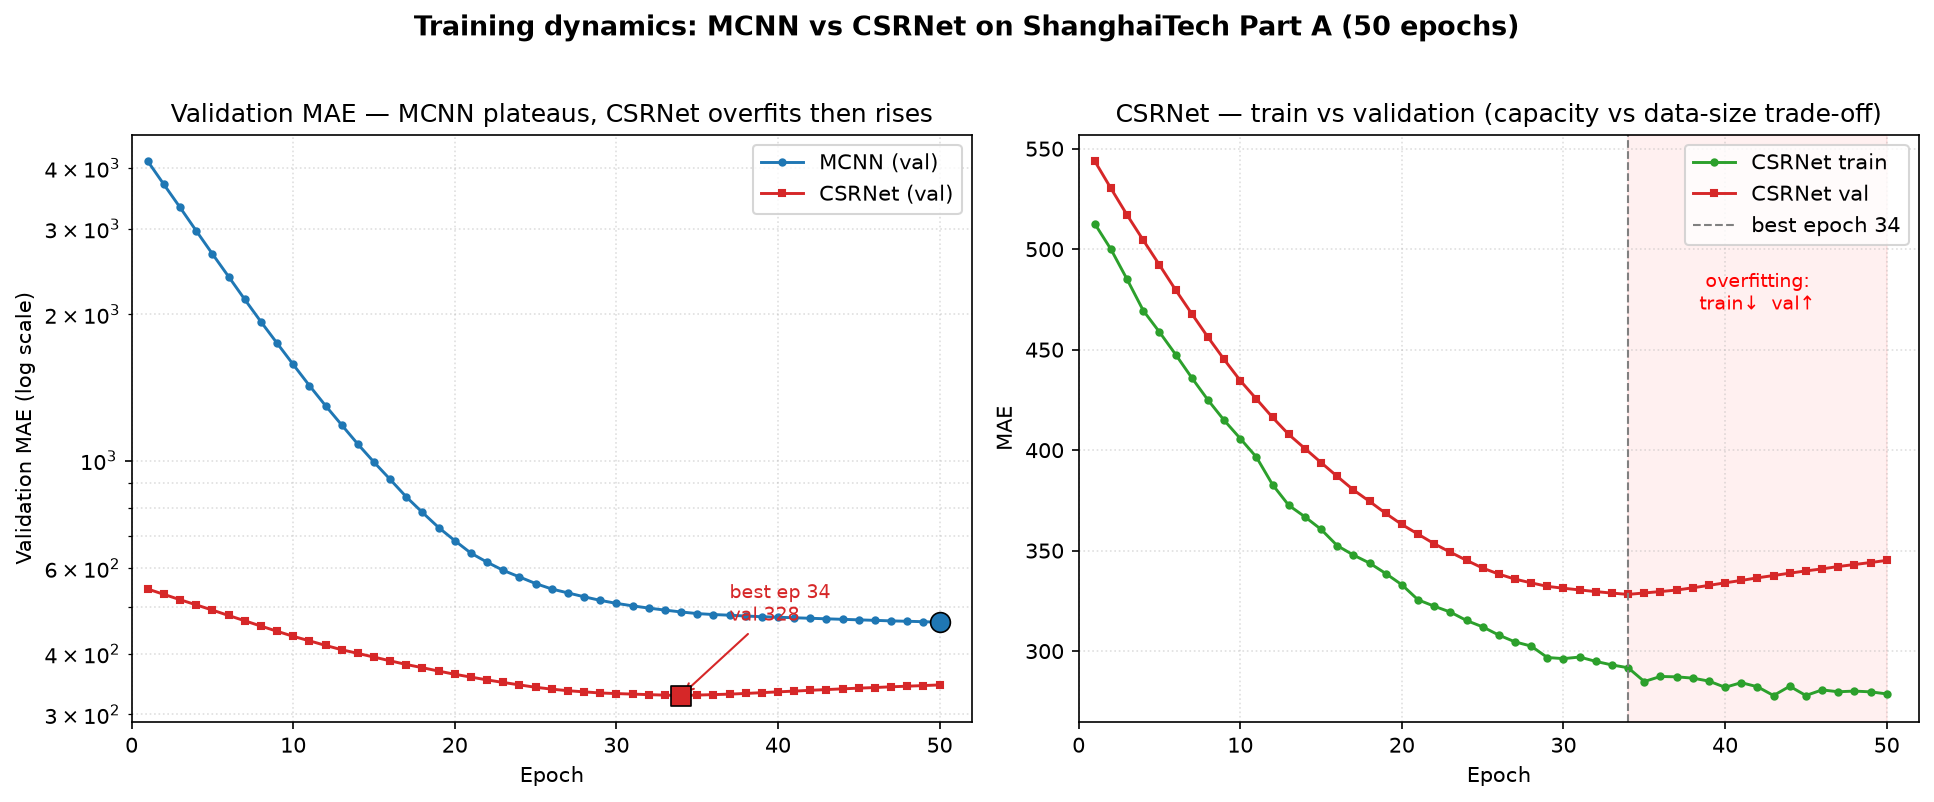
\includegraphics[width=0.62\textwidth]{figures/training_curves.png}
        \caption{Krive greške tokom treniranja (train vs validation MAE)}
    \end{figure}
    
    \vspace{-0.3cm}
    \small
    \textbf{Analiza}:
    \begin{itemize}
        \item CSRNet (pretrained VGG): Brza konvergencija, ali \textbf{overfitting} posle epohe 34 (val MAE raste, train MAE opada)
        \item MCNN (from scratch): Sporija konvergencija, stabilno do kraja, ali na višem nivou greške
    \end{itemize}
\end{frame}

% Slide 8: Gap Analysis
\begin{frame}{Analiza: Razlika u odnosu na originalne radove}
    \begin{table}
        \centering
        \begin{tabular}{@{}lcc|cc@{}}
            \toprule
            & \multicolumn{2}{c|}{\textbf{Naš rezultat}} & \multicolumn{2}{c}{\textbf{Originalni rezultat}} \\
            \textbf{Model} & MAE & RMSE & MAE & RMSE \\
            \midrule
            MCNN & 315 & 429 & $\sim$110 & $\sim$173 \\
            CSRNet & 217 & 343 & $\sim$68 & $\sim$106 \\
            \bottomrule
        \end{tabular}
    \end{table}
    
    \vspace{0.3cm}
    \textbf{Razlozi odstupanja} (sistematski, ne utiču na poređenje):
    \begin{itemize}
        \item Nema augmentacije podataka (random crops, flips)
        \item Nema learning rate scheduling
        \item Fiksna $\sigma$ (umesto adaptivne)
        \item Manji broj epoha (50 vs. više stotina)
    \end{itemize}
    
    \textbf{Važno}: Relativni odnos je isti kao u literaturi (CSRNet < MCNN).
\end{frame}

% Slide 9: Conclusion
\begin{frame}{Zaključak}
    \begin{itemize}
        \item \textbf{CSRNet superiorniji} od MCNN za brojanje u gustim gužvama na ShanghaiTech Part A
        \item Tradeoff kapaciteta i veličine skupa podataka:
        \begin{itemize}
            \item Veliki model (CSRNet, 16M) brže uči ali overfituje na malom datasetu (300 slika)
            \item Mali model (MCNN, 64K) sporiji ali stabilniji
        \end{itemize}
        \item Validnost metodologije: Poređenje pod identičnim uslovima eliminiše uticaj pipeline-a
        \item \textbf{Budući rad}:
        \begin{itemize}
            \item Augmentacija podataka (kritično za CSRNet)
            \item Adaptivna $\sigma$ za mapu gustine
            \item Learning rate scheduling i duži trening
        \end{itemize}
    \end{itemize}
    
    \vspace{0.5cm}
    \centering
    Hvala na pažnji!
\end{frame}

\end{document}
